\documentclass{article}
\usepackage[utf8]{inputenc}
\usepackage{mathtools}
\usepackage{amsmath}

\title{REA1121, Hand in 3}
\author{Nataniel Gåsøy, 131390          16HBPROGA}
\date{March 2017}

\usepackage{natbib}
\usepackage{graphicx}

\begin{document}

\maketitle
%\newline

\begin{abstract}
This is the third hand in of REA1121, mathemathics for programmers.
\end{abstract}
\vspace{10pt}

\section{Task 1}
\textbf{1.}
\textit{
u = \begin{bmatrix} 1\\  2\\ 3  \end{bmatrix}
, v = \begin{bmatrix}-3\\ 1\\ 2\end{bmatrix}
, w = \begin{bmatrix}2\\ -3\\ 1\end{bmatrix}
}
\vspace{10pt}

\textit{
Compute u + v + w and u + v + w.}
\newline
\begin{bmatrix} 1\\  2\\ 3  \end{bmatrix}
+\begin{bmatrix}-3\\ 1\\ 2\end{bmatrix}
+\begin{bmatrix}2\\ -3\\ 1\end{bmatrix}
=\begin{bmatrix}1-3+2\\ 2+1-3\\ 3+2+1\end{bmatrix}
=\begin{bmatrix}0\\ 0\\ 6\end{bmatrix}
\newline

\textit{
How do you know u + v + w lie in a plane?)}
\newline
\newline
\vspace{10pt}
We know they lie in a plane because the resulting vector lie in the 3D space.

\textit{
Alternative interpretation: How do you know u, v, w lie in a plane?)}
\newline
\vspace{10pt}
Three vectors are in the same plane if (and only if) they are linearly dependent. therefore,
if we have the values x, y, z and we can calculate x*u+y*v+z*w and get a non-zero answer,
they are not linearly independent and thus exist in the same plane. 

\textbf{2.}
\textit{
v = \begin{bmatrix} 1\\ 1 \end{bmatrix}
, w = \begin{bmatrix}1\\ 5\end{bmatrix}
}
\vspace{10pt}

\textit{
choose a number c so that w − cv is perpendicular
to v. Then find the formula that gives the number c for any
non-zero v and w.}
\newline
\newline
\vspace{10pt}
if v*w = 0, they are orthogonal. this is because cos 90 = 0.
we need to find (w-cv)*v=0
\newline
(\begin{bmatrix}1\\ 5\end{bmatrix}
- c \begin{bmatrix} 1\\ 1 \end{bmatrix}) * 
\begin{bmatrix} 1\\ 1 \end{bmatrix} = 0
\newline
w-cv = \begin{bmatrix}1\\ 5\end{bmatrix} - \begin{bmatrix}c\\ c\end{bmatrix} = 
\begin{bmatrix}1 - c\\ 5 - c\end{bmatrix}
\newline
\begin{bmatrix}1 - c\\ 5 - c\end{bmatrix} * \begin{bmatrix}1\\ 1\end{bmatrix} = 0\newline
1 - c + 5 - c = 0\newline
2c = 6\newline
\textbf{c = 3}\newline
\newline
\textit{The formula}
\newline
$
(w-cv)*v=0\newline
wv-cv^2=0\newline
wv = cv^2\newline
\frac{wv}{v^2} = c\newline$
\textbf{$\frac{w}{v} = c$}\newline


\textbf{3.}

\textit{
If $||v|| = 5$ and $||w|| = 3$, what are the smallest and largest values of $||v - w||$? What are the smallest and largest values of $||v * w||$?
$}
\newline
\newline
\vspace{10pt}
$\sqrt{v1^2*v2^2}=||v||=5$
$\sqrt{w1^2*w2^2}=||w||=3$
\newline
\textbf{$||v − w||$}\newline
We find the smallest value when they are parallel: 5 - 3 = \textbf{2}\newline
we find the largest value when they are anti-parallel: 5+3 = \textbf{8}\newline
\newline
\textbf{$||v * w||$}\newline
$||v * w|| cos &\X\theta= v * w $\newline
when they are antiparallel, cos 180 = -1. \newline
We find the largest value when they are parallel: 5*3*1 = \textbf{15}\newline
If the value can't be negative, then the lowest value is when they are orthogonal: 5*3*0 = 0
(because cos90 = 0)\newline
We find the smallest value when they are anti-parallell: 5*3*-1 = \textbf{-15}\newline

\section{Task 2}
\textbf{1.}
\textit{Let P be the plane in R3 with equation x + y − 2z = 4. Is P a subspace?
Why? Find two vectors in P and check if their sum is in P.}\newline
\newline
If we set x = 0, y = 0, z = 0 then $x+y-2+z \neq 4.$ Therefore, P is not a subspace as it
does not go through origin.\newline
\vspace{10pt}
\textit{Find 2 vectors in P:}\newline
P1: x = 1, y = 1, z = -1. $1+1-2*(-1)=4$\newline
P2: x = 6, y = 4, z = 3. $6+4-2*3=4$
P1 + P2 = \begin{bmatrix} 1+6\\ 1+4\\ 2*-1+3 \end{bmatrix} = $7+5-4=8$\newline
The sum of these two vectors are not in P.\newline

\textbf{2.}
\textit{ Construct a 3 × 3 matrix whose column space contains \begin{bmatrix} 1\\ 1\\ 0
\end{bmatrix}.
and \begin{bmatrix} 1\\ 0\\ 1 \end{bmatrix}, but not \begin{bmatrix} 1\\ 1\\ 1
\end{bmatrix}. Construct a 3 × 3 matrix whose column space is only a line.
 }
\newline
\begin{bmatrix} 1 & 1 & 0\\ 1 & 0 & 0\\ 0 & 1 & 0 \end{bmatrix} \newline
\begin{bmatrix} 1\\ 1\\ 1 \end{bmatrix} is not a linear combination of \begin{bmatrix} 1\\
1\\ 0 \end{bmatrix} and \begin{bmatrix} 1\\ 0\\ 1 \end{bmatrix}\newline
\vspace{20pt}\newline
\begin{bmatrix} 1 & 2 & 1\\ 0 & 0 & 0\\ 0 & 0 & 0 \end{bmatrix}\newline 
Here, the column space is a line (the X axis) as the others have no value/ are 0.\newline

\textbf{3.}
\textit{ Choose three independent columns of u =\begin{bmatrix} 2 & 3 & 4 & 1\\ 
0 & 6 & 7 & 0\\0 & 0 & 0 & 9\\0 & 0 & 0 & 0\\ \end{bmatrix} }\newline
The easiest way to find three independent columns of u is to use the pivot columns.
\begin{bmatrix} 2\\ 0\\ 0\\ 0 \end{bmatrix} 
\begin{bmatrix} 3\\ 6\\ 0\\ 0 \end{bmatrix} 
\begin{bmatrix} 1\\ 0\\ 9\\ 0 \end{bmatrix}\newline
\vspace{20pt}\newline

\section{Task 3}
\textbf{1.}
\textit{Are these pairs of vectors orthonormal or only orthogonal or only independent?\newline
\vspace{20pt}\newline
\textbf{a)} \begin{bmatrix} 1 \\ 0 \end{bmatrix} and \begin{bmatrix} -1 \\ 1 \end{bmatrix} 
\textbf{b)} \begin{bmatrix} 0.6 \\ 0.8 \end{bmatrix} and \begin{bmatrix} 0.4 \\
-0.3 \end{bmatrix} 
\textbf{c)} \begin{bmatrix} cos&\X\theta \\ sin&\X\theta \end{bmatrix} and 
\begin{bmatrix} -sin&\X\theta \\ cos&\X\theta \end{bmatrix}\newline}
\newline\vspace{20pt}

\textbf{a)} \begin{bmatrix} 1 \\ 0 \end{bmatrix} * \begin{bmatrix} -1 \\ 1 \end{bmatrix}
$= 1 * -1 + 0 * 1 = -1$.\newline
\textbf{The dot product here is not 0, so they are not orthogonal.} 
\newline\vspace{20pt}

\textbf{b)} \begin{bmatrix} 0.6 \\ 0.8 \end{bmatrix} * 
\begin{bmatrix} 0.4 \\ -0.3 \end{bmatrix}  
$= 0.6 * 0.4 + 0.8 * (-0.3) = 0$\newline
The dot product is 0, so they are orthogonal.\newline
$||\begin{bmatrix} 0.6 \\ 0.8 \end{bmatrix}|| = \sqrt{0.6^2 + 0.8^2 = 1}$\newline
$||\begin{bmatrix} 0.4 \\ -0.3 \end{bmatrix}|| = \sqrt{0.4^2 + (-0.3)^2 = 0.5}$\newline
\textbf{Both of these magnitudes are not 1, so they are not orthonormal.}
\newline\vspace{20pt}

\textbf{c)} \begin{bmatrix} cos&\X\theta \\ sin&\X\theta \end{bmatrix} * 
\begin{bmatrix} -sin&\X\theta \\ cos&\X\theta \end{bmatrix}\newline
$= cos&\X\theta * -sin&\X\theta + sin&\X\theta * cos&\X\theta = 0$\newline
The dot product is 0, so they are orthogonal.\newline
$||\begin{bmatrix} cos&\X\theta \\ sin&\X\theta \end{bmatrix}|| = 
\sqrt{cos&\X\theta^2 + sin&\X\theta^2 = 1}$\newline
$||\begin{bmatrix} -sin&\X\theta \\ cos&\X\theta \end{bmatrix}|| = 
\sqrt{-sin&\X\theta^2 + cos&\X\theta^2 = 1}$\newline
\textbf{Both magnitudes are 1, so these are orthonormal.}
\newline\vspace{20pt}

\textbf{2.}
\textit{A =\begin{bmatrix} 1 & 0 \\ 2 & 1\\0 & 1 \end{bmatrix}.\newline
Suppose P1 is the projection matrix onto the 1-dimensional
subspace spanned by the first column of A. Suppose P2 is the projection
matrix onto the 2-dimensional column space of A. Compute the product
P2P1.}\newline\vspace{20pt}

First column of A: \begin{bmatrix} 1 \\ 2\\0 \end{bmatrix}\newline
$P1 = \frac{aa^t}{a^ta}$\newline
$\frac{ \begin{bmatrix} 1 \\ 2\\0 \end{bmatrix}*\begin{bmatrix} 1 & 2& 0 \end{bmatrix}}
{ \begin{bmatrix} 1 & 2& 0 \end{bmatrix}* \begin{bmatrix} 1 \\ 2\\0 \end{bmatrix}}$ = 
\begin{bmatrix} 1*1 & 1*2 & 1*0 \\ 2*1 & 2*2 & 2*0\\0*1 & 0*2 & 0*0 \end{bmatrix} = 
\begin{bmatrix} 1 & 2 & 0 \\ 2 & 4 & 0\\0 &0 & 0 \end{bmatrix} * \frac{1}{5} = 
$\begin{bmatrix} \frac{1}{5} & \frac{2}{5} & 0 \\ \frac{2}{5} & \frac{4}{5} & 0\\
0 & 0 & 0 \end{bmatrix}$

column space of A: \begin{bmatrix} 1 \\ 2 \\ 0 \end{bmatrix} + 
\begin{bmatrix} 0 \\ 1 \\ 1 \end{bmatrix} = 
\begin{bmatrix} 1 \\ 3 \\ 1 \end{bmatrix}\newline
$P2 = \frac{aa^t}{a^ta}$\newline
$\frac{\begin{bmatrix} 1 \\ 3 \\ 1 \end{bmatrix}*\begin{bmatrix} 1 & 3 & 1 \end{bmatrix}}
{\begin{bmatrix} 1 & 3 & 1 \end{bmatrix} * \begin{bmatrix} 1 \\ 3 \\ 1 \end{bmatrix}}$ = 
\begin{bmatrix} 1*1 & 1*3 & 1*1 \\ 3*1 & 3*3 & 3*1\\1*1 & 1*3 & 1*1 \end{bmatrix} = 
\begin{bmatrix} 1 & 3 & 1 \\ 3 & 9 & 3\\1 & 3 & 1 \end{bmatrix} * $\frac{1}{11}$ =
\begin{bmatrix} \frac{1}{11} &  \frac{3}{11} &  \frac{1}{11} \\  
\frac{3}{11} &  \frac{9}{11} &  \frac{3}{11}\\ 
\frac{1}{11} &  \frac{3}{11} &  \frac{1}{11} \end{bmatrix}\newline

P2P1=\begin{bmatrix} \frac{1}{11} &  \frac{3}{11} &  \frac{1}{11} \\  
\frac{3}{11} &  \frac{9}{11} &  \frac{3}{11}\\ 
\frac{1}{11} &  \frac{3}{11} &  \frac{1}{11} \end{bmatrix}\ * 
$\begin{bmatrix} \frac{1}{5} & \frac{2}{5} & 0 \\ 
\frac{2}{5} & \frac{4}{5} & 0\\0 & 0 & 0 \end{bmatrix}$ = 
$\begin{bmatrix} \frac{7}{55} & \frac{14}{55} & 0 \\ 
\frac{21}{55} & \frac{42}{55} & 0\\
\frac{7}{55} & \frac{42}{55} & \frac{7}{55} \end{bmatrix}$=
\begin{bmatrix} 7 & 14 & 0 \\ 21 & 42 & 0\\7 & 14 & 0 \end{bmatrix} * $\frac{1}{55}$
\newline\vspace{20pt}

\textbf{3.}
\textit{b = \begin{bmatrix} 0 \\ 8 \\ 8 \\ 20\end{bmatrix} and 
t = \begin{bmatrix} 0 \\ 1 \\ 3 \\ 4\end{bmatrix}\newline
write down the four equations Ax = b such
that the solution fits the line b = C + Dt. Is there an exact solution? If
not, find the least squares solution xˆ such that Axˆ = p.}\newline

A = \begin{bmatrix} 1 & 0 \\ 1 & 1 \\ 1 & 3 \\ 1 & 4\end{bmatrix}
Ax = b \begin{bmatrix} 1 & 0 \\ 1 & 1 \\ 1 & 3 \\ 1 & 4\end{bmatrix} x = 
\begin{bmatrix} 0 \\ 8 \\ 8 \\ 20\end{bmatrix}\vspace{20pt}\newline

$c + d * 0 = 0$\newline
$c + d * 1 = 8$\newline
$c + d * 3 = 8$\newline
$c + d * 4 = 20$\newline
- Vector b does not lie in the column space of A.\newline
- More equations than unknown.\newline
\textbf{Ax=b is not solvabe!}
\newline\vspace{10pt}

\textit{Least square solution, \^{x} (A\^{x}=P)}\newline
A^tA\^{x}=A^tb\newline
\^{x}=(A^tA)^-1 * A^tb\newline

A^tA:\begin{bmatrix} 1 & 1 & 1 & 1 \\ 0 & 1 & 3 & 4\end{bmatrix} * 
\begin{bmatrix} 1 & 0 \\ 1 & 1 \\ 1 & 3 \\ 1 & 4\end{bmatrix} =
\begin{bmatrix} 4 & 8 \\ 8 & 26 \end{bmatrix}\newline

A^tb: \begin{bmatrix} 1 & 1 & 1 & 1 \\ 0 & 1 & 3 & 4\end{bmatrix} * 
\begin{bmatrix} 0 \\ 8 \\ 8 \\ 20\end{bmatrix} = 
\begin{bmatrix} 36 \\ 112\end{bmatrix}\newline

\begin{bmatrix} 4 & 8 \\ 8 & 26 \end{bmatrix} * \^{x} = 
\begin{bmatrix} 36 \\ 112\end{bmatrix}\newline

Gauss elimination: 
\begin{bmatrix} 4 & 8 & 36\\ 8 & 26 & 112 \end{bmatrix} $\frac{R1}{4}$ ~=
\begin{bmatrix} 1 & 2 & 9\\ 8 & 26 & 112 \end{bmatrix} R2-8R1 ~=
\begin{bmatrix} 1 & 2 & 9\\ 0 & 10 & 40 \end{bmatrix} $\frac{R2}{10}$ ~=
\begin{bmatrix} 1 & 2 & 9\\ 0 & 1 & 4 \end{bmatrix} R1-2R2 ~=
\begin{bmatrix} 1 & 0 & 1\\ 0 & 1 & 4 \end{bmatrix}\newline\vspace{10pt}
x1 = c = 1\newline
x2 = d = 4
\newline\vspace{10pt}

A\^{x}=P\newline
P = \begin{bmatrix} 1 & 0 \\ 1 & 1 \\ 1 & 3 \\ 1 & 4\end{bmatrix} * 
\begin{bmatrix} 1  \\ 4\end{bmatrix} = 
\begin{bmatrix} 1 \\ 5 \\ 13 \\ 17\end{bmatrix}\newline

\textit{Metod 1: }\newline
E = $||Ax - b||^2$\newline
(C + Dt1-b1)^2 + (C + Dt2-b2)^2 + ..... + (C + Dtn - bn)^2\newline
$(1+4*0-0)^2 + (1+4*1-8 )^2 + (1+4*3-8 )^2 + (1+4*4-20 )^2 = 1+9+25+9 = 44$\newline

\textit{Metod 2: }\newline
e = b - P\newline
\begin{bmatrix} 0 \\ 8 \\ 8 \\ 20\end{bmatrix} - 
\begin{bmatrix} 1 \\ 5 \\ 13 \\ 17\end{bmatrix} = 
\begin{bmatrix} -1 \\ 3 \\ -5 \\ 3\end{bmatrix}\newline
$(-1)^2 + 3^2 + (-5)^2 + 3^2 = 44$
e = 44\newline

\textbf{The least error, E = 44}

\section{Task 4}
this problem was hard to answer, as i do not know matlab or have much familiarity with
principal component analysis. The following answers rely heavily on what i could figure out
through google searches and wikipedia (see references).
\vspace{10pt}

\textit{The Matlab code (eigenface.m) available at Fronter
\newline(https://fronter.com/hig/links/link.phtml?idesc=1&iid=1646528) performs Principal
Component Analysis on the face images, and reproduce the images with
the k most significant principal components to represent 90% of the total
variance of all face images. Run and look through the matlab code. For
each step, explain clearly what is being computed. And figure out what the
four figures illustrate. Also you may observe the influence of the number
of principal components on the reproduced images by changing the value
of k (Line 29). For further information, please visit the Wikipedia page
of eigenface (https://en.wikipedia.org/wiki/Eigenface).}
\vspace{10pt}

\begin{verbatim}
nIMG = 40; % number of face images
for i = 1 : nIMG
    I(:,:,i) = double(imread(['\\tsclient\C\faces/',int2str(i),'.bmp'])); % Read the images
end
\end{verbatim}
Here, the code simply goes through and reads in all values of the picture files into a
single vector each.
\vspace{10pt}

\begin{verbatim}
figure(1);
imshow(reshape(EX,m,n),[]); % The "Mean" face
title('The mean face');
\end{verbatim}
Here, the code sets this figure to be figure number one.
after this, it goes through all the values of the pictures in order to get the principal
components. these are a set of values of linearly uncorrelated variables. it then compares
these values, and shows a picture of the average of these values from the pictures (mean
centering). 
Lastly, it sets the title to 'The mean face'.
\vspace{10pt}

\begin{verbatim}
figure(2);
for i = 1 : 40
    subplot(5,8,i);
    imshow(reshape(Q(:,i),m,n),[]); % The eigenfaces
    title(['Eigenface ',int2str(i)]);
end
\end{verbatim}
The purpose here is to find the eigenfaces, the sets of eigenvectors of the images.
Here, the code sets this figure to be figure number two.
then we loop through all the images. 
It next uses subplot to position the pictures. 
next, the code:
\begin{verbatim}
(Q(:,i),m,n),[])
\end{verbatim}
This subtracts the mean picture, as seen in figure number 2, from all of the original
images. 
The eigenvectors are then calculated ( of the covariance matrix).These eigenvectors have the
same number of componements as the original image, and thus they compose a new covariance
matrix. This matrix is called the eigenfaces (the directions in which the images differ from
the mean image), which is what that is displayed in figure 2.
Lastly, it sets the title to 'Eigenface ' and the picture number.
\vspace{10pt}

\begin{verbatim}
figure(3),
for i = 1 : 40
    subplot(5,8,i);
    imshow(I(:,:,i),[]); % The original faces
    title(['Face ',int2str(i)]);
end
\end{verbatim}
The purpose here is to show the original images.
Here, the code sets this figure to be figure number three.
It next uses subplot to position the pictures. 
Then it goes through and shows all the data for the images (displays the images).
As the images have been reduced to single vectors, only the most important information has
been stored. Therefore, the quality of the images is somewhat lower, but fully recognizable.
Lastly, it sets the title to 'Face ' and the picture number.
\vspace{10pt}

\begin{verbatim}
figure(4),
for i = 1 : 40
    subplot(5,8,i);
    imshow(I2(:,:,i),[0 255]);  % The reproduced faces
    title(['rpdFace ',int2str(i)]);
end
\end{verbatim}
The purpose here is to show the reproduced images.
Here, the code sets this figure to be figure number four.
It next uses subplot to position the pictures. 
This function only displays the eigenvectors for each image between 0 and 255. This means
that much information is lost. This loss is reduced by the fact that we keep the ones with
the largest eigenvalues. In other words, we keep those eigenvectors with most significance
to the picture, and discard those with the least significance. This gives us pictures with a
somewhat reduced quality but that takes much less space.
Lastly, it sets the title to 'rdpFace ' and the picture number.
\vspace{10pt}
%\begin{figure}[h!]
%\centering
%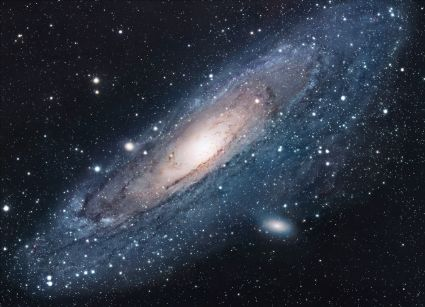
\includegraphics[scale=1.7]{universe.jpg}
%\caption{The Universe}
%\label{fig:univerise}
%\end{figure}




\section{Mathlab code}
\begin{verbatim}
%% Eigen faces
clear all
close all
clc

nIMG = 40; % number of face images
for i = 1 : nIMG
    I(:,:,i) = double(imread(['faces/',int2str(i),'.bmp'])); % Read the images
end

[m,n,~] = size(I);
X = reshape(I,[],nIMG)';
EX = mean(X,1);
B = X-ones(nIMG,1)*EX;
C = B'*B/(m*n-1);
[Q, D] = eig(C);
[d, IX] = sort(diag(D),'descend');
Q = Q(:,IX);

p = size(Q,2);
r = 1;
j = p + 1;
while r >= 0.9
    j = j - 1;
    r = sum(d(1:j))/sum(d);
end
L = j + 1;

k = L;
P = Q(:,1:k)'*B';
Xr = Q(:,1:k)*P;
I2 = reshape(Xr+EX'*ones(1,nIMG),m,n,[]);

figure(1);
imshow(reshape(EX,m,n),[]); % The "Mean" face
title('The mean face');

figure(2);
for i = 1 : 40
    subplot(5,8,i);
    imshow(reshape(Q(:,i),m,n),[]); % The eigenfaces
    title(['Eigenface ',int2str(i)]);
end

figure(3),
for i = 1 : 40
    subplot(5,8,i);
    imshow(I(:,:,i),[]); % The original faces
    title(['Face ',int2str(i)]);
end

figure(4),
for i = 1 : 40
    subplot(5,8,i);
    imshow(I2(:,:,i),[0 255]);  % The reproduced faces
    title(['rpdFace ',int2str(i)]);
end   
\end{verbatim}

\bibliographystyle{plain}
\bibliography{references}
http://www.math.colostate.edu/~clayton/teaching/m215s10/homework/hw5solutions.pdf\newline
http://math.mit.edu/~gs/linearalgebra/ila0403.pdf\newline
https://www.ucl.ac.uk/~ucahmdl/LessonPlans/Lesson10.pdf\newline
https://en.wikipedia.org/wiki/Principalcomponentanalysis.\newline
https://en.wikipedia.org/wiki/Eigenface.\newline
https://en.wikipedia.org/wiki/Covariancematrix\newline
http://image.diku.dk/shark/sphinxpages/build/html/restsources/tutorials/algorithms/pca.html
\newline

\end{document}
